\chapter{Method}
In this section, we outline the methodologies employed to develop and evaluate our PINN-models. The experiments are structured into two main parts: simulations using simple geometries and simulations based on an MRI-derived geometry. Initially, we use one-dimensional (1D) cable and two-dimensional (2D) square grid setups to generate synthetic data, providing a controlled environment to benchmark our models and compare them with previously published work \cite{EP-PINNs}. We then extend our approach to more complex and anatomically accurate heart models derived from MRI-data, capturing the intricacies of cardiac tissue structure and fiber orientation. All PINN were implemented in PyTorch~\cite{pytorch}.
The parameters used in the Aliev-Panfilov model, adopted from the original paper by Aliev and Panfilov \cite{R-D-PANFILOV20191}, are summarized in Table \ref{tab:aliev-panfilov-parameters}.

\begin{table}[h!]
    \centering
    \caption{Aliev-Panfilov Model Parameters}
    \begin{tabular}{|c|c|}
        \hline
        \textbf{Parameter} & \textbf{Value} \\
        \hline
        $\mu_1$ & 0.2 \\
        $\mu_2$ & 0.3 \\
        $k$ & 8.0 \\
        $a$ & 0.15 \\
        $b$ & 0.15 \\
        $\epsilon$ & 0.002 \\
        \hline
    \end{tabular}
    \label{tab:aliev-panfilov-parameters}
\end{table}

\section{1D Cable and 2D square geometry}\label{data_structured}
To reproduce and build upon the research presented in \cite{EP-PINNs}, we generate $\textit{in-silico}$ cardiac EP data to train and evaluate our models using two simple geometries: a 1D cable and a 2D structured square grid. 
\subsection{Synthetic Data Generation}

We generated \textit{in-silico} cardiac electrophysiological (EP) data, which served as the training and evaluation dataset. This is done by approximating the second derivatives using a central finite difference and employing a 4th-order Runge-Kutta (RK4) iterative scheme, as shown in Alg.(\ref{algo:Runge-Kutta}), for the time evolution. We impose no-flux Neumann boundary conditions in both cases.



The spatial domain was discretized using a uniform grid spacing $h$:
\begin{itemize}
  \item For the 1D case, the second spatial derivative was approximated using the central difference method:
  \begin{equation}
  \frac{\partial^2 V}{\partial x^2} \approx \frac{V_{i-1} - 2V_i + V_{i+1}}{h^2}
  \end{equation}
  where $V_i$ is the value of $V$ at the $i$-th grid point.
  \item For the 2D case, the Laplacian $\nabla^2 V$ was approximated using:
  \begin{equation}
  \nabla^2 V \approx \frac{V_{i-1,j} + V_{i+1,j} + V_{i,j-1} + V_{i,j+1} - 4V_{i,j}}{h^2}
  \end{equation}
  where $V_{i,j}$ is the value of $V$ at the grid point $(i,j)$.
\end{itemize}

Additionally, we constructed additional data sets with added noise sampled from a normal distribution with standard deviation $\sigma$.

\begin{algorithm}[H]
\caption{Fourth-Order Runge-Kutta (RK4) Method for Aliev-Panfilov Model}
\label{algo:Runge-Kutta}
\begin{algorithmic}
    \Procedure{Runge-Kutta 4th order}{}
    \State Define $f(V, W)$ and $g(V, W)$ \Comment{Right-hand sides of the differential equations}
    \State $\Delta t \leftarrow$ time step size
    %
    \For {$i = 1, 2, \ldots, n$} \Comment{Loop over time steps}
    \State $k_1V \leftarrow \Delta t \cdot f(V_i, W_i)$
    \State $k_1W \leftarrow \Delta t \cdot g(V_i, W_i)$
    \State $k_2V \leftarrow \Delta t \cdot f\left(V_i + \frac{k_1V}{2}, W_i + \frac{k_1W}{2}\right)$
    \State $k_2W \leftarrow \Delta t \cdot g\left(V_i + \frac{k_1V}{2}, W_i + \frac{k_1W}{2}\right)$
    \State $k_3V \leftarrow \Delta t \cdot f\left(V_i + \frac{k_2V}{2}, W_i + \frac{k_2W}{2}\right)$
    \State $k_3W \leftarrow \Delta t \cdot g\left(V_i + \frac{k_2V}{2}, W_i + \frac{k_2W}{2}\right)$
    \State $k_4V \leftarrow \Delta t \cdot f\left(V_i + k_3V, W_i + k_3W\right)$
    \State $k_4W \leftarrow \Delta t \cdot g\left(V_i + k_3V, W_i + k_3W\right)$
    \State $V_{i+1} \leftarrow V_i + \frac{1}{6}(k_1V + 2k_2V + 2k_3V + k_4V)$
    \State $W_{i+1} \leftarrow W_i + \frac{1}{6}(k_1W + 2k_2W + 2k_3W + k_4W)$
    \EndFor
    \EndProcedure
\end{algorithmic}
\end{algorithm}
%\subsection{Architecture and optimization}
%The architecture of the Physics-Informed Neural Network (PINN) used in this study was designed with multiple hidden layers and neurons to ensure adequate capacity for learning complex dynamics. For both the 1D cable and 2D square simulations, the PINN models were implemented in PyTorch\cite{pytorch}.

%For the 1D cable simulations, the PINN model consisted of 4 hidden layers, each containing 32 neurons. The input to the model was a 2-dimensional vector $(x, t)$ representing the spatial and temporal coordinates, and the output was a 2-dimensional vector $(\tilde{V}, \tilde{W})$ corresponding to the state variables in the Aliev-Panfilov model. The hyperbolic tangent (\texttt{tanh}) activation function was used due to its smooth and differentiable nature, which is beneficial for solving partial differential equations (PDEs)\cite{experts}.

%For the 2D square simulations, the PINN model had 5 hidden layers with 64 neurons each. The input to the model was a 3-dimensional vector $(x, y, t)$, representing the spatial coordinates in two dimensions and the temporal coordinate. The output was the same 2-dimensional vector $(V, W)$.

%The optimization of the model parameters was performed using the Adam optimizer. For the 1D model, the learning rate was set to $0.005$ with a weight decay of $1 \times 10^{-3}$, and an exponential learning rate scheduler with a decay rate of $0.98$ was employed. The 2D model was optimized with a learning rate of $0.0005$, and an exponential learning rate scheduler with a decay rate of $0.98$ was used. Both models were trained for a sufficient number of epochs to ensure convergence, specifically a maximum of $20,000$ epochs for the 1D model and $50,000$ epochs for the 2D model. 


\subsection{Evaluation}
In order to evaluate the performance, we calculated the root mean squared error (RMSE) across the evaluation points as outlined in \cite{EP-PINNs}.
\begin{equation}
RMSE = \sqrt{\frac{1}{n} \sum_{i=1}^n (\tilde{V}_i - V_{\text{ref}_i})^2}   
\end{equation}

To investigate the variability of the models, we trained 10 distinct models for each combination of training sample sizes (\(n = 10^2, 10^3, 10^4\)) and noise levels (\(\sigma = 0.0, 0.01, 0.1\)). We calculated the RMSE values for each model and reported the interquartile range (IQR) to measure the variability in the predictions. The IQR, representing the middle $50\%$ of the RMSE values, provided an insight into the consistency of model performance across different training scenarios.



\section{MRI based geometry}\label{method_MRI}
In this section, we present the methodology concerning more complex and anatomically accurate 2D geometries derived from MRI data. 
\subsection{Synthetic Data generation for the MRI based geometry}

As shown in Figure \ref{fig:mri}, a computational model was derived from a late gadolinium-enhanced MRI 2D-slice acquired from  from the Royal Brompton Hospital, using a previously described protocol \cite{gulati}. 

\begin{figure}[h]
  \centering
  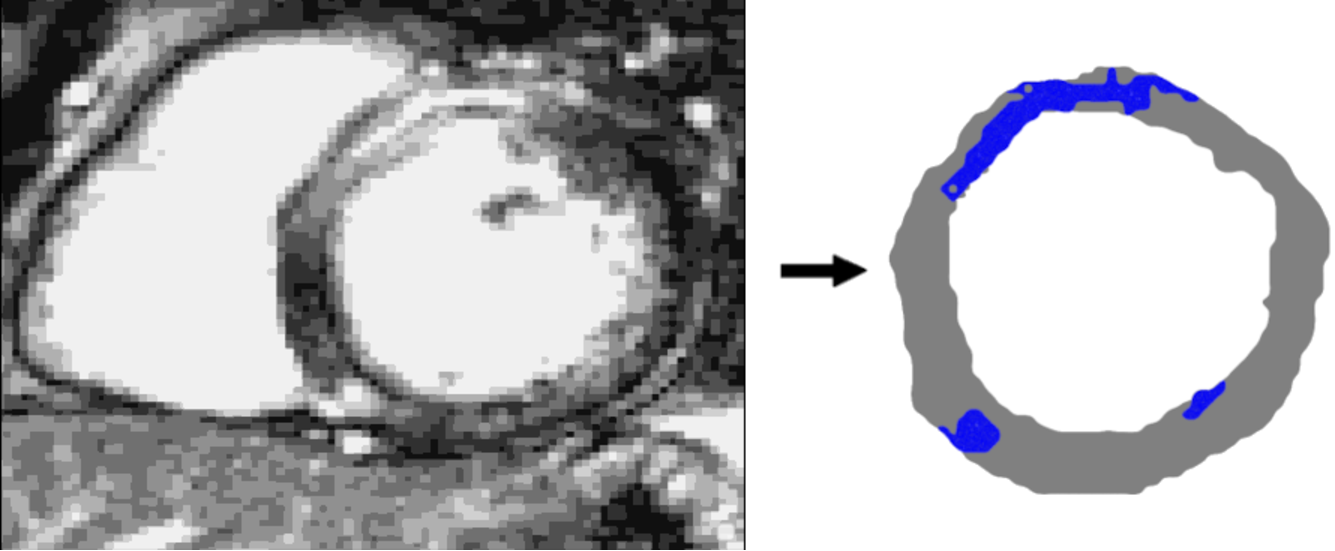
\includegraphics[width=0.7\textwidth]{Figs/Anisotropic/MRI_to_model.pdf}
  \caption{Generation of a Computational Heart Model from MRI Data. The left panel shows a raw 2D MRI slice. The right panel presents the resulting computational model that has been extracted from the MRI data, where the blue region marks an area with scar tissue and reduced conductivity.}
  \label{fig:mri}
\end{figure}
We generate a computational mesh composed of triangles with edge length of $250\mathrm~{\mu s}$ consisting of $72434$ vertices. The image processing and mesh generation methodologies are outlined in detail by Balaban et al. \cite{balaban}.
We carried out FEM simulations using openCARP~\cite{openCARP-sw} under both isotropic and anisotropic conditions with an initial stimulus given by a circular pulse with strength $500 \mathrm{\mu A/cm^2}$ with a duration of $2\mathrm{\mu s}$. The simulations were carried out using a time step of $20\mathrm{\mu s}$, with $V_m$ and $W$ outputed every $5\mathrm{ms}$ for a total of $211$ time steps. The simulations all consiststed of a single heartbeat with a duration of $1050\mathrm{ms}$. 
In the isotropic conductivity scenario the longitudinal and transverse conductivities were as shown in Table \ref{tab:Isotropic_g}. 
\begin{table}[h]
  \centering
  \begin{tabular}{|c|c|}
    \hline
    Parameter & Value \\ \hline
    $g_{et}$ & 1 \\ \hline
    $g_{it}$ & 1 \\ \hline
    $g_{il}$ & 0.2 \\ \hline
    $g_{it}$ & 0.2 \\ \hline
  \end{tabular}
  \caption{Isotropic conductivities}
  \label{tab:Isotropic_g}
\end{table}

Under anisotropic conditions, the data was generated from multiple FEM simulations with fixed extracellular conductivities (\(g_{el} = 1~\mathrm{S/m}\), \(g_{et} = 1~\mathrm{S/m}\)) and intracellular transverse conductivity (\(g_{it} = 1~\mathrm{S/m}\)), while varying intracellular longitudinal conductivity (\(g_{il}\)) from 0.5 to 1 in steps of 0.05. Addtionally, MRI-derived scar tissue is introduced into the computational model as conductive heterogeneities in the regions marked in blue in Figure \ref{fig:mri}, with conductivities as shown in Table \ref{tab:scar}. 
\begin{table}[H]
  \centering
  \begin{tabular}{|c|c|}
    \hline
    Parameter & Value \\ \hline
    $g_{il}$ & $0.0775~\mathrm{S/m}$ \\ \hline
    $g_{it}$ & $0.0143~\mathrm{S/m}$ \\ \hline
    $g_{el}$ & $0.2785~\mathrm{S/m}$ \\ \hline
    $g_{et}$ & $0.0512~\mathrm{S/m}$ \\ \hline
  \end{tabular}
  \caption{Conductivities in the scar region.}
  \label{tab:scar}
\end{table}


\subsection{Fibers}


%Cardiomyocytes are joined to form long fibers, where excitation is faster along the fibers(longitudonal direction) than perpendicular(transverse direction). As such, the orientation of these fibers determines the direction of electrical wave propagation and accurate modeling of these structures is crucial to obtain accurate simulations. 

In the heart muscle, cardiomyocytes are interconnected to form elongated fibers, wherein excitation propagates more rapidly longitudinally than in the transverse direction \cite{conduction_direction}. Consequently, the orientation of these fibers determines the preferred direction of electrical wave propagation in the heart. Thus precise modeling to approximate these configurations is essential for achieving accurate simulations which reflect biological reality within pre-defined tolerance. We inferred fiber orientations from MRI using a widely-used rule-based method described in \cite{Bayer2012}. 

The fiber orientations are initially defined for each triangle in the generated computational mesh. To translate this rotational data to the points used in a PINN, we employ a local averaging approach. For each target vertex, all triangles containing that vertex are identified. The fiber field at each point is then calculated by averaging the fiber fields of the neighboring triangles, weighted by the area of each triangle:
\[
e_f (\text{point}) = \sum_{\text{neighboring triangles } i} \text{area}(\text{triangle}_i) \cdot e_f(\text{triangle}_i)
\]
Finally, the fiber vector at each point is normalized.


Assuming that the intracellular and extracellular conductivity tensors are given by
\begin{equation}
\Sigma_i = \begin{bmatrix} g_{il} & 0 \\ 0 & g_{it} \end{bmatrix}
\end{equation}
and
\begin{equation}
\Sigma_e = \begin{bmatrix} g_{el} & 0 \\ 0 & g_{et} \end{bmatrix},
\end{equation}
where $g_{il}$ is the longitudinal intracellular conductivity,  $g_{it}$ is the transverse intracellular conductivity and similarly for the extracellular conductivities $g_{el}$ and $g_{el}$.

We can calculate the local conductivity tensors $\tilde{\Sigma_i}, \tilde{\Sigma_e}$
by means of the local fiber vector $e_f(x,y)$ using tensor rotation. We define the local rotation tensor 
\begin{align} 
R = \begin{bmatrix} e_f^x & e_f^y \\  -e_f^y & e_f^x \end{bmatrix}
\end{align}
so that
\begin{align}
\tilde{\Sigma_i} &= R \Sigma_i R^T\\
\tilde{\Sigma_e} &= R \Sigma_e R^T \\
\end{align}

and finally
\begin{equation}
\Sigma_m = \tilde{\Sigma_i} \tilde{\Sigma_e} (\tilde{\Sigma_i} + \tilde{\Sigma_e})^{-1}.
\end{equation}


%\textcolor{red}{fibres are defined per triangle in the FEM sim. The PINN uses a point cloud, so we need to translate the rotation data to points. We do this by averaging the fiber fields by triangle area.}




\subsection{Boundary normals}
In the context of calculating normals when training a PINN, it is important to remember that we are dealing with a point cloud rather than a continuous surface. 
Considering that the normal of a point isn't well defined, we need to resort to an approximation. 
Given a point \( \mathbf{P} \) and its two nearest neighbors \( \mathbf{N}_1 \) and \( \mathbf{N}_2 \), the line segment between the neighboring points, \( \mathbf{l} \), is given by

\[
\mathbf{l} = \mathbf{N}_1 - \mathbf{N}_2.
\]
We can then approximate the boundary normal vector at point \( \mathbf{P} \) as the normal vector of \( \mathbf{l} \).
This can be done by using the cross product of \( \mathbf{l} \) with a unit vector orthogonal to the plane of interest (in this case, the \( z \)-axis unit vector \( \mathbf{k} = [0, 0, 1] \)) such that

\[
\mathbf{n} = \mathbf{l} \times \mathbf{k}
\]

The resulting normal vector \( \mathbf{n} \) is then projected onto the \( xy \)-plane by discarding its \( z \)-component:

\[
\mathbf{n}_{xy} = [n_x, n_y].
\]

The orientation of the normal vector is then adjusted based on whether the point is on the inner or outer boundary. 


Finally, all normal vectors were normalized to unit length:

\[
\mathbf{n}_{xy} = \frac{\mathbf{n}_{xy}}{\|\mathbf{n}_{xy}\|}.
\]



\begin{comment}
\[
\mathbf{n}_{xy} = \begin{cases} 
-\mathbf{n}_{xy} & \text{if } \mathbf{P} \in \text{inner boundary} \\
\mathbf{n}_{xy} & \text{if } \mathbf{P} \in \text{outer boundary}
\end{cases}
\]
\subsubsection{Non-Dimensionalization}

\textcolor{red}{Note: explain ww want to do this(activation function non-linearity and NN performance when inputs are scaled PDE-loss needs to be scaled)}\\
We have 

\begin{equation}
\label{eq:dvdt}
    \frac{\partial V}{\partial t}=\nabla \cdot (\mathbf{\sigma}_m \nabla V) - kV(V-a)(V-1)-VW,
\end{equation}
and
\begin{equation}
\label{dwdt}
    \frac{\partial W}{\partial t}= (\epsilon + \frac{\mu_1W}{V+\mu_2})(-W-kV(V-b-1)).
\end{equation}
\\

Rescaling $x$,$y$ and $t$ such that

\begin{equation}
    \Tilde{x}=\alpha x,\: \Tilde{y}=\alpha y,\: \text{and}\: \Tilde{t}=\beta t,
\end{equation}



where $\alpha$ and $\beta$ are constant scaling factors, we get



\begin{equation}
    \frac{\partial x}{\partial \Tilde{x}} = \frac{1}{\alpha},\: \frac{\partial y}{\partial \Tilde{y}} = \frac{1}{\alpha}\: \text{and}\: \frac{\partial t}{\partial \Tilde{t}} = \frac{1}{\beta}.
\end{equation}

Using the chain rule, we get

\begin{equation}
    \frac{\partial V}{\partial \Tilde{x}}=\frac{\partial x}{\partial \Tilde{x}}\frac{\partial V}{\partial x} \rightarrow \frac{\partial V}{\partial x}=\alpha \frac{\partial V}{\partial \Tilde{x}},
\end{equation}

\begin{equation}
    \frac{\partial V}{\partial \Tilde{y}}=\frac{\partial y}{\partial \Tilde{y}}\frac{\partial V}{\partial y} \rightarrow \frac{\partial V}{\partial y}= \alpha \frac{\partial V}{\partial \Tilde{y}},
\end{equation}
and 
\begin{equation}
    \frac{\partial V}{\partial \Tilde{t}}=\frac{\partial t}{\partial \Tilde{t}}\frac{\partial V}{\partial t} \rightarrow \frac{\partial V}{\partial t} = \beta \frac{\partial V}{\partial \Tilde{t}}.
\end{equation}
\\

Similarly, we get $\frac{\partial \sigma(x,y)}{\partial x} = \alpha \frac{\partial \sigma(x,y)}{\partial \Tilde{x}}$ and $\frac{\partial \sigma(x,y)}{\partial y} = \alpha \frac{\partial \sigma(x,y)}{\partial \Tilde{y}}$.\\

Thus, we can write \eqref{eq:dvdt} and \eqref{dwdt} as
\begin{equation}
\label{eq:dvdt}
    \beta \frac{\partial V}{\partial \Tilde{t}}=\alpha^2\Tilde{\nabla} \cdot (\mathbf{\sigma}_m \Tilde{\nabla} V) - kV(V-a)(V-1)-VW,
\end{equation}
and
\begin{equation}
\label{dwdt}
    \beta \frac{dW}{d \Tilde{t}}= (\epsilon + \frac{\mu_1W}{V+\mu_2})(-W-kV(V-b-1)).
\end{equation}
\end{comment}



\subsection{Evaluation}
In evaluating the performance of our MRI-based models, we employ the relative $L^1$ norm, $RL^1$, defined as

\begin{equation}
RL^1 = \frac{\sum_{i} |\tilde{V}_i - V_i|}{\sum_{i} |V_i|},
\end{equation}
where $\tilde{V}_i$ and $V_i$ are the PINN approximated solution and the reference FEM solution, respectively. 
We also consider the relative $L^2$ error, $RL^2$, for comparison with existing literature \cite{PDL}, which is defined as
\begin{equation}
RL^2 = \frac{\sqrt{\sum_{i} (\tilde{V}_i - V_i)^2}}{\sqrt{\sum_{i} V_i^2}}.
\end{equation}

The relative \( L^1 \) error provides a scale-invariant assessment of model performance, ensuring that errors are evaluated proportionally to the magnitude of the targets. The relative \( L^1 \) error is less sensitive to slight phase shifts as compared to the relative \( L^2 \) norm, making it more robust in scenarios where small temporal misalignments might otherwise result in disproportionately large error values.
\newpage
\section{Optimization}



\subsection{Adam Optimizer}
In order to find the optimal parameters $\theta^*$, we need to minimize \eqref{eq:pinn_loss}. One of the most commonly used optimization algorithms in training PINNs is Adaptive Moment Estimation (Adam)~\cite{adam}. Adam is an extension of the stochastic gradient descent (SGD) algorithm that computes adaptive learning rates for each parameter. The algorithm maintains two moving averages for each parameter: the first moment and the second moment. These moments are used to adapt the learning rates of the parameters, which helps in converging more quickly and avoiding local minima more effectively. These properties make Adam a preferred choice for training complex neural network architectures such as PINNs \cite{experts}. For more details on the Adam optimizer, the reader can refer to the original paper by Kingma and Ba \cite{adam}.






\begin{algorithm}[H]
\caption{Adam Optimizer \cite{adam}}
\label{alg:Adam}
\begin{algorithmic}[1]
\State \textbf{Initialize:}
\Statex \hspace{1em} $\theta_0$ \hfill (initial parameters)
\Statex \hspace{1em} $m_0 = 0$ \hfill (first moment vector)
\Statex \hspace{1em} $v_0 = 0$ \hfill (second moment vector)
\Statex \hspace{1em} $t = 0$ \hfill (time step)
\Statex \hspace{1em} $\eta$ \hfill (learning rate)
\Statex \hspace{1em} $\beta_1 = 0.9$ \hfill (decay rate for first moment)
\Statex \hspace{1em} $\beta_2 = 0.999$ \hfill (decay rate for second moment)
\Statex \hspace{1em} $\epsilon = 10^{-8}$ \hfill (small constant to prevent division by zero)
\While{not converged}
    \State $t = t + 1$
    \State $g_t = \nabla_{\theta} L(\theta_{t-1})$ \hfill(compute gradients of the loss function $L$ w.r.t. $\theta$)
    \State $m_t = \beta_1 m_{t-1} + (1 - \beta_1) g_t$ \hfill(update biased first moment estimate)
    \State $v_t = \beta_2 v_{t-1} + (1 - \beta_2) g_t^2$ \hfill(update biased second moment estimate)
    \State $\hat{m}_t = m_t / (1 - \beta_1^t)$ \hfill(compute bias-corrected first moment estimate)
    \State $\hat{v}_t = v_t / (1 - \beta_2^t)$ \hfill(compute bias-corrected second moment estimate)\
    \State $\theta_t = \theta_{t-1} - \alpha \hat{m}_t / (\sqrt{\hat{v}_t} + \epsilon)$ \hfill(update parameters)
\EndWhile
\State \textbf{return} $\theta_t$
\end{algorithmic}
\end{algorithm}
\subsection{Learning rate decay}
The choice of learning rate is arguably the most important hyperparameter in training neural networks, as it significantly influences the convergence speed and the quality of the final model \cite{LR}\cite{Goodfellow}. An appropriate learning rate ensures efficient progress in the loss landscape, while an excessively high learning rate can cause the training process to overshoot minima or even diverge, and a too-low learning rate can result in a prolonged training process that might get stuck in suboptimal local minima \cite{Goodfellow}.

In the context of using the Adam optimizer, which adjusts the learning rate for each parameter based on the first and second moments of the gradients, the learning rate parameter $\eta$ acts as an approximate upper bound on the effective step size \cite{adam}. To optimize the training process, we employed an exponential learning rate scheduler as suggested in \cite{experts}, which systematically decreases the learning rate $\eta$ over the course of training. This scheduler is implemented in PyTorch and follows the formula $\eta_t = \eta_0 \cdot \exp(-\gamma t)$, where $\eta_0$ is the initial learning rate, $\gamma$ is the decay rate, and $t$ represents the epoch or iteration number.



\section{Input scaling}\label{scaling}
Scaling of neural network inputs (in our case physical quantities) is an important step in training neural networks, ensuring that these inputs (features) contribute equally to the learning process. Differences in scales of features or very large features can lead to several issues that negatively impact model performance.

Firstly, features with larger scales can dominate the learning process, causing features with smaller scales to be effectively ignored. This imbalance can skew the model's predictions and reduce its overall performance \cite{Goodfellow}. 

Secondly, large feature values can saturate activation functions, particularly those like the sigmoid or tanh functions, which are prone to saturation. When these functions saturate, their gradients approach zero. This issue significantly hampers the learning process, as the model updates the weights very slowly \cite{glorot}.



In one commonly used scaling approach, feature scaling is performed as a preprocessing step before training the neural network \cite{experts}. Consequently, the differential equations governing the physics of the problem must be scaled accordingly to maintain consistency when evaluating the residuals given by \eqref{eq:R_V} and \eqref{eq:R_W}.

An alternative approach (which we have not seen in PINN litterature) involves scaling the features within the network itself, making the scaling operation part of the computational graph so that the residuals of the governing equations are evaluated correctly. This can be achieved in two ways: by using a frozen scaling layer (fixed parameters) or by incorporating scaling as the first step in the forward pass.
We introduce a scaling layer, which offers the added benefit of storing the scaling factors together with the model's optimal parameters, simplifying the process for future inference.
We employ min-max scaling, which transforms each feature individually so that they are within a given range $[a,c]$:  
\begin{equation}
    x'=a + \frac{x -\text{min}(x)(c-a)}{\text{max}(x) -\text{min}(x)},
    \label{eq:min_max_single}
\end{equation}
where $x'$ is the scaled feature $x$, while $\text{max}(x)$ and $\text{min}(x)$ denote that largest and smallest values of the specific feature in the training set.

Let $\Vec{x} \in \mathbb{R}^i$ denote the inputs, where $i$ is the number of input nodes. If $\Vec{x}_{\text{max}}\in \mathbb{R}^i$ and $\Vec{x}_{\text{min}}\in \mathbb{R}^i$ are the feature wise largest and smallest values respectively, then we can rescale the inputs by
\begin{equation}
    \vec{x}'=\vec{a} + (x -\Vec{x}_{\text{min}})\odot(\vec{c}-\vec{a})\oslash  (\Vec{x}_{\text{max}}-\Vec{x}_{\text{min}}),
    \label{eq:min_max}
\end{equation}

where $\vec{x}'$ is the rescaled inputs, $\odot$ is element-wise multiplication and $\oslash$ is element-wise division. Each element of $\Vec{a} \in \mathbb{R}^i$ and $\Vec{c} \in \mathbb{R}^i$ have values $a$ and $c$ respectively.
Now, let $W_s \in \mathbb{R}^{i\times i}$ be the weights matrix of the scaling layer and $\vec{b}_s\in \mathbb{R}^i$ be the bias. We then want our outputs from the scaling layer to be the rescaled inputs given by \eqref{eq:min_max} such that

\begin{equation}
    W_s\Vec{x} +\vec{b}_s=\vec{a} + (x -\Vec{x}_{\text{min}})\odot(\vec{c}-\vec{a})\oslash  (\Vec{x}_{\text{max}}-\Vec{x}_{\text{min}}).
    \label{eq:min_max}
\end{equation}

Re-arranging the right-hand side, we get


\begin{equation}
 W_s\Vec{x} +\vec{b}= \Vec{x}\oslash\left[\Vec{x}_{\text{max}}-\Vec{x}_{\text{min}}\right] + \left[\Vec{a} - \Vec{x}_{\text{min}}\odot(\vec{c}-\vec{a})\oslash  (\Vec{x}_{\text{max}}-\Vec{x}_{\text{min}})\right].
\end{equation}
We then see that $W_s$ must be a diagonal matrix where the diagonal is given by 

\begin{equation}
\text{diag}(W_s)=\Vec{1}\oslash\left[\Vec{x}_{\text{max}}-\Vec{x}_{\text{min}}\right],
\end{equation}
and the bias is given by
\begin{equation}  
\Vec{b}_s=\left[\Vec{a} - \Vec{x}_{\text{min}}\odot(\vec{c}-\vec{a})\oslash  (\Vec{x}_{\text{max}}-\Vec{x}_{\text{min}})\right].
\end{equation}

\section{Multi-Objective Loss balancing}\label{loss_balance}
\begin{comment}
    
The hybrid loss function defined in \ref{eq:pinn_loss} belongs to the category of Multi-Objective Optimization, where many components have different units of measurement, which inevitably creates a disparity in their magnitudes. This can lead to an imbalance where some loss components dominate the optimization process, favoring the components with the highest magnitude. To address this issue, we introduce a loss balancing scheme based on Relative Loss Balancing with Random Lookback (ReLoBRaLo)\cite{ReLoBRaLo}. Consider $n$ loss terms $\mathcal{L}_i$, where $i \in \{1,\dots,n\}$. In order to ensure that each term progresses at a similar rate, we employ a relative loss balancing strategy. The key idea is to adjust the weighting of each loss term according to its relative progress since the start of training. Let $\mathcal{L}_i(t)$ denote the value of the $i$-th loss term at training iteration $t$, and $\mathcal{L}_i(0)$ its value at the beginning of training. 

We define the progress of each loss term as:
\begin{equation}
\alpha_i(t) = \frac{\mathcal{L}_i(t)}{\mathcal{L}_i(0)}, \quad i \in \{1, \dots, n\}
\end{equation}

The greater the progress since the beginning of training, the smaller the value of $\alpha_i(t)$ will be. This is desirable, as we want to assign higher weights to loss terms that have shown less progress, and lower weights to those that have already improved significantly.

To achieve this, we use $\alpha_i(t)$ as the weighting factor for each loss term based on their relative progress:
\begin{equation}
\alpha_i(t) = \frac{\mathcal{L}_i(t)}{\mathcal{L}_i(0)}, \quad i \in \{1, \dots, n\}
\end{equation}



Note that this approach represents a key element of ReLoBRaLo, focusing on the relative loss balancing aspect. However, it does not include the random lookback mechanism that is part of the full ReLoBRaLo methodology.
\end{comment}
The hybrid loss function defined in \eqref{eq:pinn_loss} belongs to the category of Multi-Objective Optimization, where many components have different units of measurement, which inevitably creates a disparity in their magnitudes. This can lead to an imbalance where some loss components dominate the optimization process, favoring the components with the highest magnitude. To address this issue, a recently published study by Bischof et al. \cite{ReLoBRaLo} proposes a self-adaptive loss balancing scheme for PINNs, namely \emph{Relative Loss Balancing with Random Lookback}(ReLoBRaLo). The ReLoBRaLo method combines elements from previous adaptive loss balancing techniques and introduces new features such as random lookback and "temperature scaling" to dynamically adjust the contributions of different loss components. This results in more stable and efficient training of PINNs by preventing any single loss term from dominating the optimization process and allowing the network to achieve better overall performance.



\textbf{Initialization:} At the beginning of training, initial losses for each component are recorded. Each loss component is assigned an initial weight of 1.

\textbf{Dynamic Weight Calculation:} At each iteration, weights for the loss components are updated based on the relative changes in their respective loss values. The weight \(\lambda_i\) for each loss component \(\mathcal{L}_i\) is calculated as:
\begin{equation}
\lambda_i(t) = \alpha \lambda_i^{\text{hist}}(t) + (1 - \alpha) \lambda_i^{\text{bal}}(t, t-1),
\end{equation}

where

\begin{equation}
\lambda_i^{\text{bal}}(t, t') = k \cdot \frac{\exp \left( \frac{L_i(t)}{\tau L_i(t')} \right)}{\sum_{j=1}^k \exp \left( \frac{L_j(t)}{\tau L_j(t')} \right)},
\end{equation}
and
\begin{equation}
\lambda_i^{\text{hist}}(t) = \rho \lambda_i(t-1) + (1 - \rho) \lambda_i^{\text{bal}}(t, 0).
\end{equation}
In this context, $\lambda_i^{\text{bal}}(t, t')$ defines the scaling in accordance with the relative improvement between a previous iteration $t'$ and the current iteration $t$. In this case, $\tau$ is a temperature parameter controlling the sharpness of the softmax operation.
$\lambda_i^{\text{hist}}(t)$ determines if the scaling is calculated from the previous timestep or the improvement from the initial iteration.
\(\alpha\) is the exponential decay rate, and \(\rho\) is a Bernoulli random variable (taking values $0$ or $1$).












\section{Architecture}\label{architecture}


The architectures of the PINN models are illustrated in Figure \ref{fig:architecture} and hyperparameters for each experiments are summarized in Table \ref{table:hyperparameters}. In the case of isotropic conductivities, the network takes the spatial coordinates \( \vec{x} \) and time \( t \) as inputs.
For anisotropic and heterogeneous conductivities, the model is designed to take the components of the spatially varying local diffusion tensor (defined in \ref{mono_aliev}) as inputs in addition to spatio-temporal coordinates.

The PINNs were implemented using PyTorch\cite{pytorch}. All models utilize the Glorot uniform initialization \cite{glorot} for the weights, and biases are initialized to zero.

The network architectures used for the 1D and 2D structured geometries are adopted from \cite{EP-PINNs}, while the architectures for the MRI-based geometries were manually tuned to balance the complexity and computational efficiency. The isotropic model uses fewer layers and nodes, while the anisotropic model requires more complexity to capture locational and directional dependencies in conduction. We use the $\tanh$ activation function throughout.
%except for the anisotropic model which has a Sigmoid-weighted Linear Unit (SiLU)\cite{silu} in the last layer.
\begin{table}[ht]
\centering
\caption{Hyperparameter settings by experiment}
\resizebox{\textwidth}{!}{
\begin{tabular}{|c|c|c|c|c|}
  \hline
  \textbf{Hyperparameter} & \textbf{1D Cable} & \textbf{2D Square} & \textbf{MRI Isotropic} & \textbf{MRI Anisotropic} \\ \hline
  Max Epochs & $20000$ & $30000$ & $50000$ & $100000$ \\ \hline
  Activation & $\tanh$ & $\tanh$ & $\tanh$ & $\tanh$ \\ \hline
  Inputs & $2$ & $3$ & $3$ & $7$ \\ \hline
  Hidden Layers & $4$ & $5$ & $5$ & $7$ \\ \hline
  Nodes & $32$ & $64$ & $128$ & $[128,\dots,128,256]$ \\ \hline
  Weight Initialization & Glorot uniform & Glorot uniform & Glorot uniform & Glorot uniform \\ \hline
  $\eta$ & $5\times 10^{-3}$ & $5\times 10^{-3}$ & $5\times 10^{-4}$ & $2\times 10^{-4}$\\ \hline
  $N_c$ & $ 10^{4}$ & $ 10^{4}$ & $2\times10^{4}$ & $5\times10^{4}$\\ \hline
  $N_{BC}$ & $ 10^{2}$ & $ 10^{3}$ & $2\times10^{3}$ & $2\times10^{3}$\\ \hline

\end{tabular}
}
\label{table:hyperparameters}
\end{table}
\begin{comment}
\begin{wraptable}{r}{0.3\textwidth}
  \centering
  \caption{Hyperparameter settings for 1D model.}
  \resizebox{\linewidth}{!}{
  \begin{tabular}{|c|c|}
    \hline
    \textbf{Hyperparameter} & \textbf{Choice} \\ \hline
    Max Epochs & 20000 \\ \hline
    Activation & tanh \\ \hline
    Layers & 4 \\ \hline
    Nodes & 32 \\ \hline
    Weight initialization & Glorot uniform \\ \hline
    $\eta$ & 0.05 \\ \hline
    
  \end{tabular}
  }
    \label{table:1D_hyper}
\end{wraptable}
\begin{wraptable}{r}{0.3\textwidth}
  \centering
  \caption{Hyperparameter settings for 2D square model.}
\resizebox{\linewidth}{!}{
  \begin{tabular}{|c|c|}
    \hline
    \textbf{Hyperparameter} & \textbf{Choice} \\ \hline
    Max Epochs & 30000 \\ \hline
    Activation & tanh \\ \hline
    Layers & 5 \\ \hline
    Nodes & 64 \\ \hline
    Weight initialization & Glorot uniform \\ \hline
    $\eta$ & 0.0005 \\ \hline
    
  \end{tabular}
  }
    \label{table:2D_hyper}
\end{wraptable}
\begin{wraptable}{r}{0.2\textwidth}
\resizebox{0.65\linewidth}{!}{ 
    \begin{tabular}{|c|c|}
      \hline
      \textbf{Hyperparameter} & \textbf{Choice} \\ \hline
      Epochs & 30000 \\ \hline
      Activation & tanh \\ \hline
      Inputs & 9\\ \hline
      Hidden layers & 7 \\ \hline
      Nodes & 150 \\ \hline
      Weight initialization & Glorot uniform \\ \hline
      $\eta$ & 0.0005 \\ \hline
    \end{tabular}
    }
    \captionof{table}{Hyperparameters used for training. }
    \label{table:MRI_aniso_hyper}
\end{wraptable}
\begin{wraptable}{r}{0.2\textwidth}
  \centering
  \caption{Hyperparameter settings for 2D MRI model.}
  \resizebox{0.65\linewidth}{!}{
  \begin{tabular}{|c|c|}
    \hline
    \textbf{Hyperparameter} & \textbf{Choice} \\ \hline
    Max Epochs & 50000 \\ \hline
    Activation & tanh \\ \hline
    Layers & 5 \\ \hline
    Nodes & 128 \\ \hline
    Weight initialization & Glorot uniform \\ \hline
    $\eta$ & 0.0005 \\ \hline  
  \end{tabular}
  }
    \label{table:MRI_iso_hyper}
\end{wraptable}
\end{comment}
\begin{figure}[H]
  \centering
  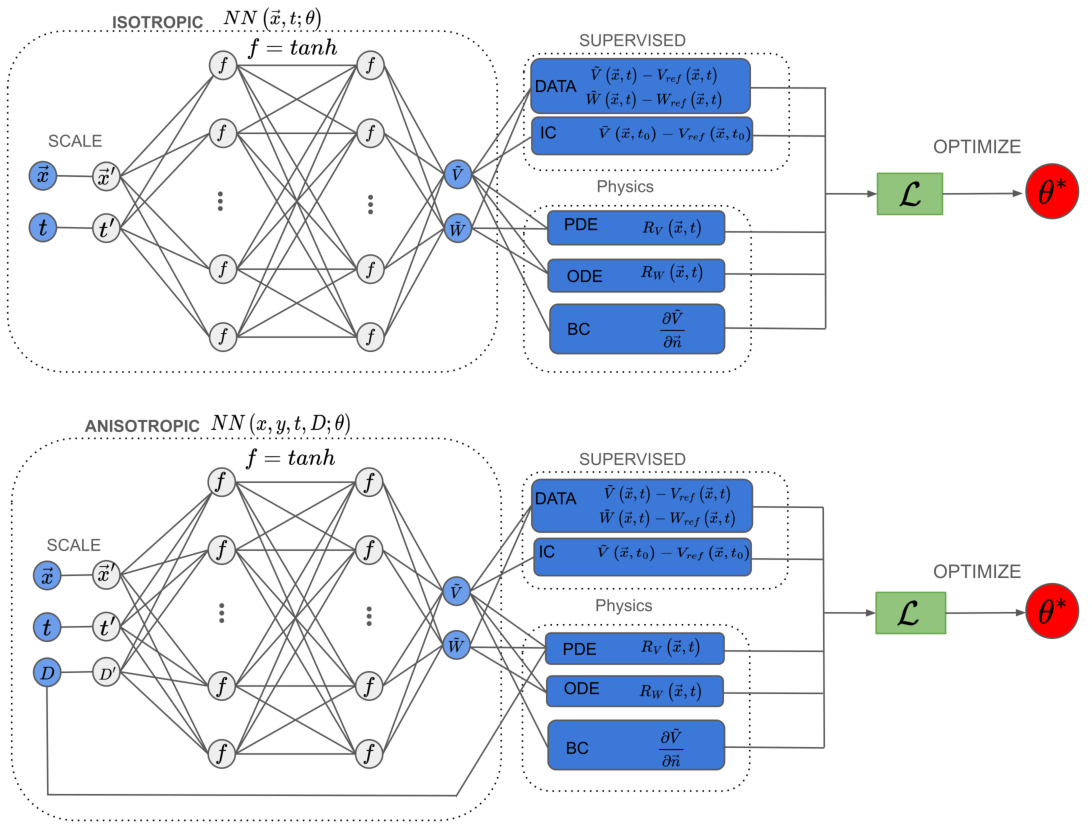
\includegraphics[width=\textwidth]{Figs/Architecture.pdf}
  \caption{Architecture of the PINNs used in this study. The top section illustrates the isotropic model, which takes spatio-temporal coordinates \(\vec{x}\) and \(t\) as inputs. The bottom section shows the anisotropic model with inputs \(x, y, t, D\). All models use tanh activation functions and include supervised learning components (DATA and IC) as well as physics-based constraints (PDE, ODE, BC). The loss function \(\mathcal{L}\) is optimized to determine the best parameters \(\theta^*\).}
  \label{fig:architecture}
\end{figure}

\section{Training Procedures}
This section outlines the training procedures employed for various models. Common in all training procedures, is the use of full-batch training, as evidence suggests that large batch sizes are best suitable for training PINNs, providing faster training times and improved accuracy \cite{batch_size}. Additionally, we use early-stopping, a form of regularization where training is stopped before overfitting happens. This is done by monitoring an appropriate metric computed across a validation dataset and saving the model with the lowest validation error as described in \cite{lu2021deepxde}. Finally, all models in this study utilize gradient clipping during training. Gradient Clipping is a commonly used heuristic~\cite{Goodfellow} to prevent excessively large gradients and has been demonstrated to accelerate the convergence of neural networks \cite{gradient_clipping}. This technique involves rescaling the gradients to a predefined threshold, maintaining their direction while diminishing their magnitude.

The differences in training procedures are mainly concerning data selection and loss balancing:
\begin{itemize}
\item For the 1D and 2D structured geometry models, we selected $n$ spatio-temporal datapoints sampled uniformly. The remaining data was split equally into validation and evaluation sets. In this experiment, all loss weights in \eqref{eq:pinn_loss} are set to one as done in \cite{EP-PINNs}.

\item In the case of the MRI-based geometry with isotropic conductivities, we sample time-series data at $n_s$ spatial locations. The remaining points were reserved for validation and evaluation (equally split). Loss weights are balanced as described in Section \ref{loss_balance}.

\item For the MRI-based geometry with anisotropic conductivities, training is done with a subset of the datasets ($g_{il}=0.5,0.6,0.7,0.8,0.9$), from which we sample $N=10^6$ spatio-temporal points for training. A validation set is also constructed by sampling $10^6$ spatio-temporal points. The selection of training data leaves the remaining conductivity scenarios for evaluating the unbiased predictive capabilities of the model outside the training range.  Loss weights are balanced as described in Section \ref{loss_balance}.
\end{itemize}

\begin{comment}
\section{Training procedures}
Outline training procedures:
-- train test split\\
In the simple geometry scenarios we sample N datapoints and leave the remaining unseen data to evaluate the model.
-- Gradient clipping\\
During the gradient descent based optimization processes, the gradients of the loss function with respect to the network parameters guide the parameter updates. Nevertheless, overly large gradients can cause instabilities in the learning process. Gradient Clipping is a commonly used heuristic~\cite{Goodfellow} to prevent excessively large gradients and has been demonstrated to accelerate the convergence of neural networks \cite{gradient_clipping}. This technique involves rescaling the gradients to a predefined threshold, maintaining their direction while diminishing their magnitude. All models in this study utilize gradient clipping during training.
-- LR scheduler:  \\
The choice of learning rate is arguably the most important hyperparameter in training neural networks, as it significantly influences the convergence speed and the quality of the final model. An appropriate learning rate ensures efficient progress in the loss landscape, while an excessively high learning rate can cause the training process to overshoot minima or even diverge, and a too-low learning rate can result in a prolonged training process that might get stuck in suboptimal local minima \cite{Goodfellow}.

In the context of using the Adam optimizer, which adjusts the learning rate for each parameter based on the first and second moments of the gradients, the learning rate parameter $\eta$ acts as an approximate upper bound on the effective step size \cite{adam}. To optimize the training process, we employed an exponential learning rate scheduler as suggested in \cite{experts}, which systematically decreases the learning rate $\eta$ over the course of training. This scheduler is implemented in PyTorch and follows the formula $\eta_t = \eta_0 \cdot \exp(-\lambda t)$, where $\eta_0$ is the initial learning rate, $\lambda$ is the decay rate, and $t$ represents the epoch or iteration number.

The exponential decay of the learning rate helps in achieving faster convergence and avoids overshooting the optimal solution by gradually reducing the learning rate. This allows the optimizer to make finer adjustments as training progresses, thereby improving convergence stability and model performance \cite{loshchilov2016sgdr, goodfellow2016deep}.

-- Scaling\\
Feature scaling is a crucial preprocessing step in training neural networks, ensuring that the features contribute equally to the learning process. Differences in scales of features can lead to several issues that negatively impact model performance.

Firstly, features with larger scales can dominate the learning process, causing features with smaller scales to be effectively ignored. This imbalance can skew the model's predictions and reduce its overall performance. 

Secondly, large feature values can saturate activation functions, particularly those like the sigmoid or tanh functions, which are prone to saturation. When these functions saturate, their gradients approach zero, leading to the vanishing gradient problem. This issue significantly hampers the learning process, as the model updates the weights very slowly, if at all, during backpropagation. Consequently, the training process becomes inefficient and can get stuck, failing to converge to an optimal solution.


When implementing scaling in the context of training PINNs, there are primarily two approaches.
In the first approach, feature scaling is performed as a preprocessing step before training the neural network. Consequently, the differential equations governing the physics of the problem must be scaled accordingly to maintain consistency.

The second approach involves scaling the features within the network itself, making the scaling operation part of the computational graph. This can be achieved in two ways: by using a frozen scaling layer or by incorporating scaling as the first step in the forward pass.
We introduce a scaling layer, which offers the added benefit of storing the scaling factors together with the model's optimal parameters, simplifying the process for future inference.
We employ min-max scaling, which transforms each feature individually so that they are within a given range $[a,c]$:  
\begin{equation}
    x'=a + \frac{x -\text{min}(x)(c-a)}{\text{max}(x) -\text{min}(x)},
    \label{eq:min_max_single}
\end{equation}
where $x'$ is the scaled feature, while $\text{max}(x)$ and $\text{min}(x)$ denote that largest and smalest values of the specific feature in the training set.
Let $\Vec{x} \in \mathbb{R}^i$ denote the inputs, where $i$ is the number of input nodes. If $\Vec{x}_{\text{max}}\in \mathbb{R}^i$ and $\Vec{x}_{\text{min}}\in \mathbb{R}^i$ are the feature wise largest and smallest values respectively, then we can rescale the inputs by
\begin{equation}
    \vec{x}'=\vec{a} + (x -\Vec{x}_{\text{min}})\odot(\vec{c}-\vec{a})\oslash  (\Vec{x}_{\text{max}}-\Vec{x}_{\text{min}}),
    \label{eq:min_max}
\end{equation}

where $\vec{x}'$ is the rescaled inputs, $\odot$ is elementwise multiplication and $\oslash$ is element eise division. Each element of $\Vec{a} \in \mathbb{R}^i$ and $\Vec{c} \in \mathbb{R}^i$ hold values $a$ and $c$.
Now, let $W_s \in \mathbb{R}^{i\times i}$ be the weights matrix of the scaling layer and $\vec{b}\in \mathbb{R}^i$ be the bias. We then want our outputs from the scaling layer to be the rescaled inputs given by \ref{eq:min_max} such that

\begin{equation}
    W_s\Vec{x} +\vec{b}=\vec{a} + (x -\Vec{x}_{\text{min}})\odot(\vec{c}-\vec{a})\oslash  (\Vec{x}_{\text{max}}-\Vec{x}_{\text{min}}).
    \label{eq:min_max}
\end{equation}

Rearranging the right hand side, we get


\begin{equation}
 W_s\Vec{x} +\vec{b}= \Vec{x}\oslash\left[\Vec{x}_{\text{max}}-\Vec{x}_{\text{min}}\right] + \left[\Vec{a} - \Vec{x}_{\text{min}}\odot(\vec{c}-\vec{a})\oslash  (\Vec{x}_{\text{max}}-\Vec{x}_{\text{min}})\right].
\end{equation}
We then see that $W_s$ must be a diagonal matrix where the diagonal is given by $\text{diag}(W_s)=\Vec{1}\oslash\left[\Vec{x}_{\text{max}}-\Vec{x}_{\text{min}}\right]$, and $\Vec{b}_s=\left[\Vec{a} - \Vec{x}_{\text{min}}\odot(\vec{c}-\vec{a})\oslash  (\Vec{x}_{\text{max}}-\Vec{x}_{\text{min}})\right]$.


\end{comment}

